\chapter{Implémentation}

\section{Logiciel}
Le logiciel développer dans le cadre de ce travail à pour objectif de collecter, traiter, afficher, et sauver les données mesurer par le capteur.
Le logiciel fourni par le fabriquant permet deja d'utiliser le capteur, cependant il manque certaine fonctionnalité. Le nouveux logiciel apporte donc des fonctionnalités  importantes du logiciel, on peut citer l’ouverture dans une seule fenêtre unique, ce qui facilite la navigation et la lisibilité.
L'utilisateur a un contrôle total sur les mesures : il peut notamment ajuster la précision ainsi que la largeur de bande de la mesure (en Hz).
Il peut aussi choisir non seulement quel harmonique on désire mesurer mais il est possible de choisir plusieurs à mesurer en même temps.

\subsection{architectures du Logiciel}
Le programmes utilise une architecture orienter object. chaque object a une responsablilté voir figure \ref{uml.drawio}. L'object Serial s'occupe de la communiction avec la balace. Il est responssable de la connection, de lire les sorties et de mettre en forme les données recus.
L'object signal lui s'occupe des signeux une fois recu dans le C'est cet object qui s'occupe de faire le traitement du signal. Parameter contiens tous les paramètre pour chaque signal. L'object mesure petremet de faire le lient entre les diferent object. ilt est responsable de toute la mesure. 

\fig[H, width=12cm]{Diagramme de classe}{uml.drawio}

\subsection{Mesures}
Les mesures se déroulent en deux étapes.
Dans un premier temps, le capteur effectue une mesure de calibration. Cette mesure consiste à balayer toute la plage de fréquences allant de 1 à 5,5 MHz avec un pas entre les point de mesures de 1KHz voir figure \ref{fig:calibration plot}.
L’objectif de cette étape est d’identifier automatiquement les fréquences de résonance du quartz. Pour ce faire, il est essentiel de détecter la fréquence fondamentale du quartz afin de déterminer s’il s’agit d’un quartz 10 MHz ou 5 MHz.
La méthode consiste à repérer la position du premier pic de résonance. Une fois cette fréquence déterminée, le programme peut ensuite rechercher toutes les fréquences de résonance : on en attend trois pour un quartz à 10 MHz et six pour un quartz à 5 MHz.

\begin{figure}[H]
    \centering
    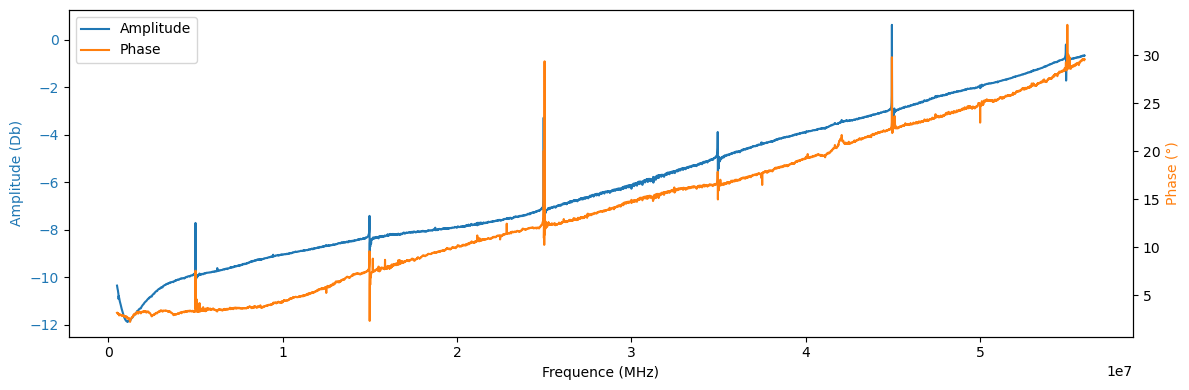
\includegraphics[width=\textwidth]{assets/figures/Calibration.png}
    \caption{Signal de calibration du capteur QCM comportant 6 pics de résonance.}
    \label{fig:calibration plot}
\end{figure}
La deuxième étape consiste à Mesurer plus précisement les pics de résonance figure~\ref{fig:harmonic plot} trouver lors de la mesure de callibration.
 Pour faire cela une fenetre est choisis autour de chaque pic de raisonnace. 
 Dans le cas de la fugure \ref{fig:harmonic plot} la fenêtre commence -5000 Hz et termine à +15000 Hz de la frequence de callibration . Le pas de mesure est de 20Hz pour une précision maximale.
\begin{figure}[H]
    \centering
    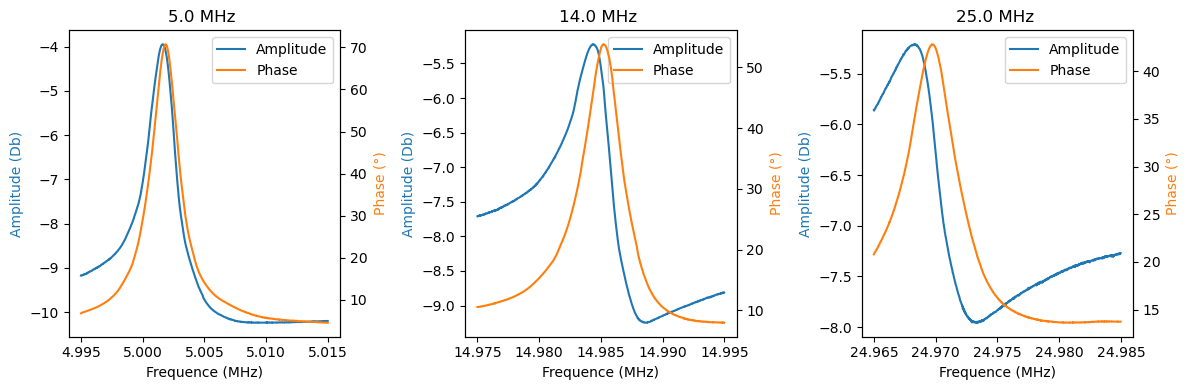
\includegraphics[width=\textwidth]{assets/figures/signalpeak.png}
    \caption{Signal des 3 premières harmoniques de résonance.}
    \label{fig:harmonic plot}
\end{figure}

\subsection{selection des mesures}
Depuis le menu il est possible d'accéder a la fenetre de sélection des paramètres de mesure voir figure\ref{fig:paramerter window}.
Les paramètres suivant peuvent être modifier par l'utilisateur celon ses besoins.
\begin{itemize}
    \item \textbf{Limite du nombre de mesures} : Le nombre maximum de mesures à effectuer. La limite peut être désactivée l'utilisateur devra alors appuyer sur stop pour arrêter la mesure.
    \item \textbf{pas de la messure de calibration} : Le pas de mesure en Hz pour la mesure de calibration.
    \item \textbf{décalage negatif de la des mesures de peak}: Le décalage négatif à appliquer aux mesures de pic.
    \item \textbf{décalage positif de la des mesures de peak}: Le décalage positif à appliquer aux mesures de pic.
    \item \textbf{pas des messures de peak} : Le pas de mesure en Hz pour les mesures de pic.
    \item \textbf{harmonique} : La ou les harmoniques à mesurer. Il est possible de sélectionner plusieurs harmoniques.
    \item \textbf{temps d'attente}: Le temps d'attente entre chaque mesure en secondes.
    \item \textbf{Calibration par la phase} : Si cette option est activée, la calibration se fera en fonction de la phase du signal. sinon la calibration se fera en fonction de l'amplitude du signal.
\end{itemize}

\begin{figure}[H]
    \centering
    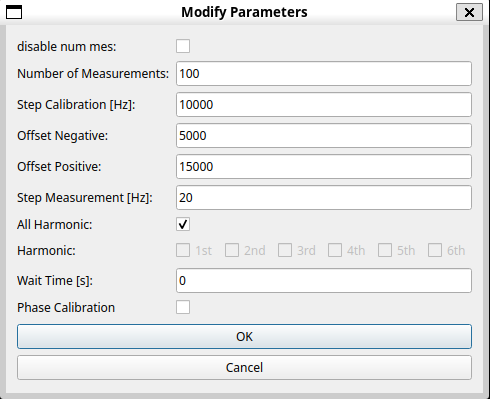
\includegraphics[width=0.6\textwidth]{assets/figures/Parameter_window.png}
    \caption{Fenêtre de selection des paramètres de mesure}
    \label{fig:paramerter window}
\end{figure}

\subsection{affichage des données}
Le logiciel dispose de plusieurs fenêtres pour afficher les données.
La première est la fenêtre de mesures figure~\ref{fig:main window} qui est composer d'une barre d'outil sur le dessus qui contiens tous les contrôles nessecaire a contrôler les mesures.
Sur la droite une liste permet de visualiser l'ensemble des baches mesurer ainsi que les paramètre associer.
A gauche une section est réserver pour les graphiques. cette zone est séparer en trois partie:
\begin{itemize}
    \item La partie supérieure affiche les signaux d'amplitude et de phase du signal de calibration.
    \item La partie centrale affiche les signaux d'amplitude et de phase des harmoniques mesurées. Ce groupe est dynamique selon le nombre d'harmoniques choisies.
    \item La partie inférieure affiche la fréquence de la première harmonique mesurée en fonction du temps. Ainsi que la température du capteur intégré.
\end{itemize}

La deuxième fenêtre est la fenêtre de visualisation des données figure~\ref{fig:plot window}. 
Elle permet de visualiser les données mesurées sous forme de graphique. 
Il est possible de choisir n'importe quelle paramètre de la mesure à afficher sur l'axe de abscisse et n'importe quel paramètre de la mesure à afficher sur l'axe des ordonnées.
Il est aussi possible de choisir l'harmonique à afficher.
\begin{figure}[H]
    \centering
    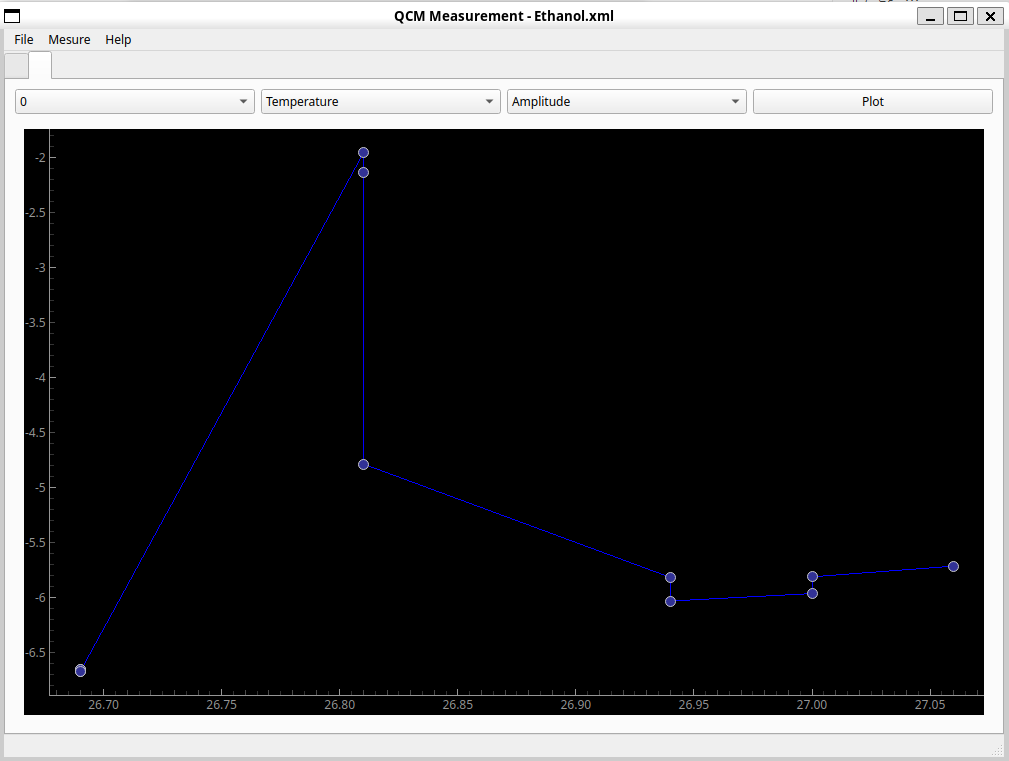
\includegraphics[width=0.8\textwidth]{assets/figures/Plot_window.png}
    \caption{Fenetre de visualisation des données}
    \label{fig:plot window}
\end{figure}
\begin{figure}[H]
    \centering
    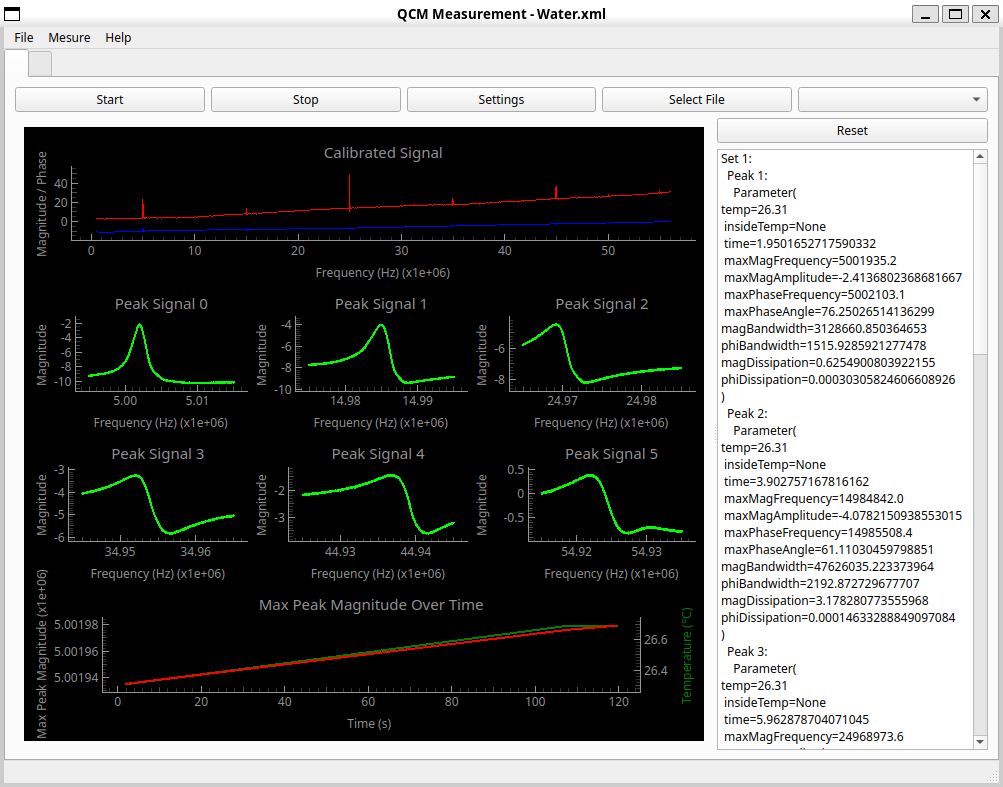
\includegraphics[width=0.8\textwidth]{assets/figures/Programme.png}
    \caption{Fenetre principale du logiciel de mesure}
    \label{fig:main window}
\end{figure}


\subsection{communication avec le capteur}
Pour communiquer avec le capteur, une connexion série est établie. Cette connexion permet d'envoyer des commandes et de recevoir des données.

L’envoi des commandes se fait au moyen d’une chaîne de caractères. La commande comprend la fréquence de début, la fréquence de fin et le pas de la mesure. Les données sont séparées par un point-virgule (;). La trame est terminée par un retour à la ligne (\texttt{\textbackslash n}).
\begin{minted}{bash}
500000;55990000;10000

9985000;10004980;20

29995000;30014980;20
\end{minted}
Le capteur répond avec les données mesurées. Les données sont formatées avec l'amplitude en premier suivi par la phase et séparées par un point-virgule (;). Les points de mesure sont séparés par un retour à la ligne (\texttt{\textbackslash n}).
pour annoncer que la mesure est terminée le capteur envoie la température en degrés Celsius suivi par un point-virgule (;) et un (s)

\begin{minted}{bash}
2968.94;3450.61\n

25.81;s
\end{minted}

La conversion des valeurs brutes issues de l'ADC en unités amplitude se fait selon l'équation~\ref{eq:adc_conversion_Amplitude}, et la phase selon l'équation~\ref{eq:adc_conversion_phase}.

\begin{equation}
A_i = \frac{\left( \left( x_i \times \frac{k}{2} \right) - V_{\text{CP}} \right)}{0.03}
\label{eq:adc_conversion_Amplitude}
\end{equation}

\begin{equation}
\phi_i = \frac{\left( \left( x_i \times \frac{k}{1.5} \right) - V_{\text{CP}} \right)}{0.01}
\label{eq:adc_conversion_phase}
\end{equation}

\begin{equation}
k = \frac{V_{\text{max}}}{N_{\text{max}}}
\label{eq:adc_conversion}
\end{equation}

où :
\begin{itemize}
    \item $x_i$ : valeur brute de l'ADC pour l'échantillon $i$,
    \item $V_{\text{max}}$ : tension maximale mesurable par l'ADC (ici $3.3\,\mathrm{V}$),
    \item $N_{\text{max}}$ : valeur maximale du codeur ADC (ici $8192$ pour un ADC sur 13 bits),
    \item $V_{\text{CP}}$ : tension de référence (0.9),
    \item $y_i$ : valeur convertie (en unité physique finale).
\end{itemize}

\section{traitement du signal}
à complèter
\newpage


\section{Sonde de température}
Le capteur QCM intègre une sonde de température juste en dessous du quartz. Cependant après avoir fait plusieurs tests avec un thermomètre, nous avons constaté que la mesure de température fournie par le capteur n'était pas toujours fiable. Des écarts de température allant jusqu'à 5 degrés Celsius ont été observés entre les deux capteurs.
Pour remédier à ce problème il a été décider d'automatiser la prise de temperature.


\begin{table}[h!]
\centering
\begin{tabular}{|p{3.5cm}|p{1.5cm}|p{1.5cm}|p{1.5cm}|p{2.5cm}|p{2cm}|p{3.5cm}|}
\hline
\textbf{Type de capteur} & \textbf{Précision} & \textbf{Linéarité} & \textbf{Temps de réponse} & \textbf{Plage (°C)} & \textbf{Coût} & \textbf{Remarques} \\
\hline
Thermistance (NTC) & ±0.2 °C à\newline ±1.0 °C & Mauvaise & Rapide & −55 à\newline +125 & Faible & Bon marché,\newline mais non linéaire \\
\hline
Thermocouple (Type K) & ±1 à\newline ±2.5 °C & Moyenne & Très rapide & −200 à\newline +1350 & Moyen & Large plage,\newline nécessite compensation \\
\hline
RTD (Pt100) & ±0.1 °C à\newline ±0.5 °C & Excellente & Moyen & −200 à\newline +850 & Élevé & Très précis,\newline mais plus coûteux \\
\hline
\end{tabular}
\caption{Comparaison de capteurs thermiques selon plusieurs critères (version compacte)}
\end{table}

Le choix s'est porter sur le capteur PT100 principalement pour sa précision et linearité. ce qui rend le Programme d'interpretation des données plus simple.
Le fonctionnement du 

\subsection{Conditionnement du signal}
Le capteur PT100 nécessite un conditionnement du signal pour convertir la variation de résistance en une tension mesurable.
Le circuit de conditionnement est composé d'un pont de Wheatstone, d'un amplificateur de tension, d'un filtre passe-bas, un Microcontrôleur est ensuite utiliser pour convertir le signal analogiquer en numerique, Le microcontrôleur transemeet egalement les données de température à l'ordinateur.

\fig[H, width=12cm]{Shéma du circuit de conditionnement}{ShemaElec.drawio}

\subsubsection{Pont de Wheatstone}
le pont de Wheatstone est un circuit utilisé pour mesurer très précisément la variation de résistance de la sonde en fonction de la température. 
Il fonctionne en comparant la Pt100 à des résistances de référence dans un montage équilibré. Toute variation de température modifie la résistance de la Pt100, 
créant un déséquilibre mesurable sous forme de tension. Cette tension différentielle est proportionnelle à la variation de température.

\subsubsection{Amplificateur de tension}
L'amplificateur de tension est composé d'un amplificateur opérationnel et d'une résistance de gain. 
Il est utilisé pour amplifier le signal de tension issu du pont de Wheatstone.
L'amplification est nécessaire pour rendre le signal suffisamment fort pour être traité par le microcontrôleur.
L'amplificateur est configuré en mode non inverseur pour garantir que le signal reste positif et proportionnel à la variation de température.
Le gain de l'amplificateur est ajusté pour correspondre à la plage de tension acceptable par le microcontôleur à savoir entre 0 et 5V.

\subsubsection{Filtre passe-bas}
Lors des premier tests de mesures de temperature, il a été constaté que le signal de température était instable.
Chaque harmonique auquel le capteur vibrais donnais une temperature différente, pour une harmonique donnée la temperature restais stable.
\begin{figure}[H]
    \centering
    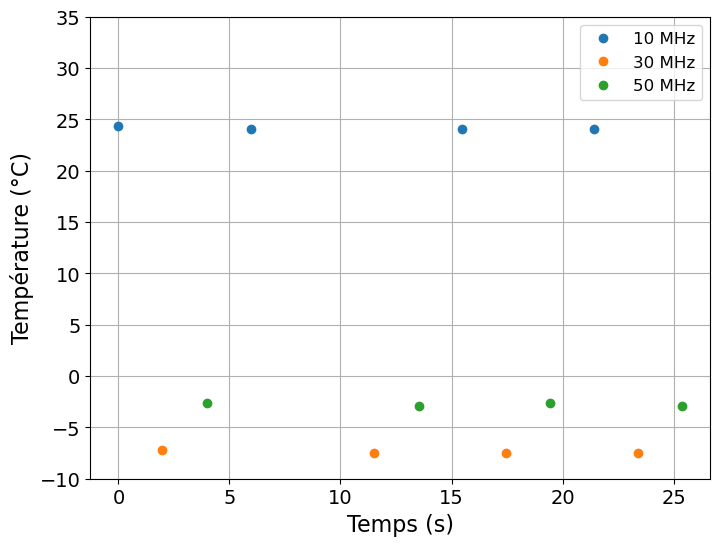
\includegraphics[width=0.8\textwidth]{assets/figures/TempBruit.png}
    \caption{Fenetre principale du logiciel de mesure}
    \label{fig:TempBruit}
\end{figure}

La plusieur piste ont été envisagées comme cause de ce problème, la sonde qui ne serais pas correctement isolée, une alimentation instable, ou encore des interférences électromagnétiques.
Les deux première piste ont été rapidement écartées, car la sonde est correctement isolée et l'alimentation est stable.
Pour verifier notre troisième hypothèse, un oscilloscope a été utilisé pour observer le signal de sortie du pont de Wheatstone.

Lors de la première harmonique il le signal à la sorte du pont de wheatstone est bruité.
Sur la figure \ref{fig:10mhzbruit} on peut lire visualiser un signal oscillatoire d'une amplitude de 8,55mv et un longeur d'onde de 32ns ce qui représente une frequence de 31,25MHz.
cette frequance est similare à celle de la 3ème harmonique du quartz de 10MHz. ce qui pourrais provenir d'un mode de raisonnance du quartz auquel il est spécialement sensible. 
il est aussi interessaant de noter que l'amplitude est la plus petite des trois mesures et que la forme de l'onde n'est pas une sinusoid contrairement aux deux autres.
\begin{figure}[H]
    \centering
    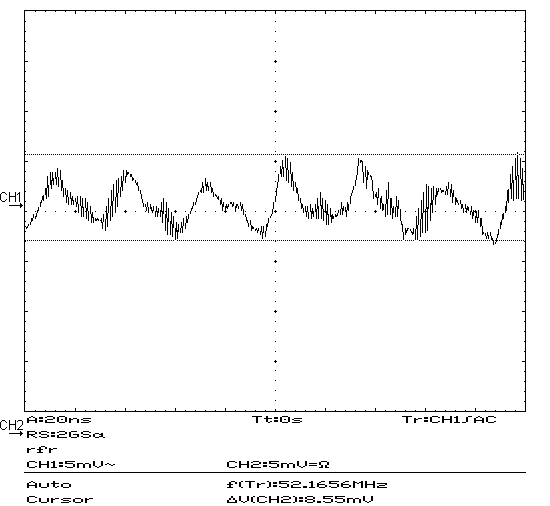
\includegraphics[width=0.8\textwidth]{assets/figures/SCR00006.png}
    \caption{Fenetre principale du logiciel de mesure}
    \label{fig:10mhzbruit}
\end{figure}

Lors de la deuxième mesure avec un le signal d'exitation de 30MHz, le signal à la sortie du pont de Wheatstone a une forme sinusoidale avec une amplitude de 21mv soit plus de du fois le signal de la première mesure et une longeur d'onde de 32ns ce qui représente une fréquence de 31,25MHz.
Cette féquance est très similaire à la frequance d'exitation du quartz. 
\begin{figure}[H]
    \centering
    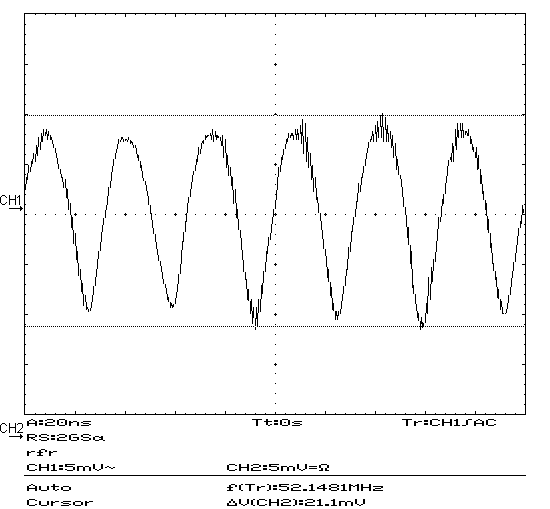
\includegraphics[width=0.8\textwidth]{assets/figures/SCR00007.png}
    \caption{Fenetre principale du logiciel de mesure}
    \label{fig:30mhzbruit}
\end{figure}

La troisième mesure avec un signal d'exitation de 50MHz, le signal à la sortie du pont de Wheatstone a une forme sinusoidale avec une amplitude de 18mV.
la lonfuer d'onde est de 20ns ce qui représente une fréquence de 50MHz ce qui correpond à la fréquence d'excitation du quartz.
\begin{figure}[H]
    \centering
    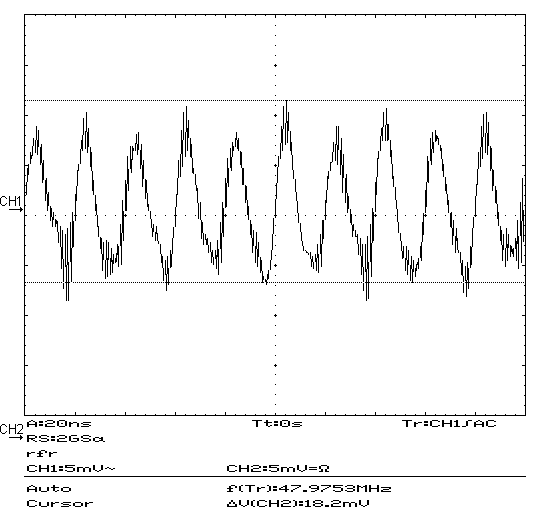
\includegraphics[width=0.8\textwidth]{assets/figures/SCR00008.png}
    \caption{Fenetre principale du logiciel de mesure}
    \label{fig:50mhzbruit}
\end{figure}

Une correlation entre l'amplitude du signal mesurer et les perturbations de mesures de temperature de la  figure \ref{fig:TempBruit} a été établie.
Cette perturbation est principalement due à la bande passante limitée de l'amplificateur opérationnel utilisé dans le circuit de conditionnement. Lorsque la fréquence du signal dépasse la bande passante de l'amplificateur, celui-ci n'est plus capable de suivre correctement les variations rapides, ce qui introduit du bruit et des distorsions dans la mesure de température.

Pour remédier à ce problème, un filtre passe-bas a été ajouté au circuit de conditionnement du signal.
Le filtre passe-bas est conçu pour atténuer les fréquences supérieures à 1 kHz, ce qui permet de réduire les interférences et de stabiliser la mesure de température.

Pour déterminer la fréquence de coupure du filtre passe-bas, on utilise la formule classique reliant la résistance $R$ et la capacité $C$ du filtre RC :

\begin{equation}
f_c = \frac{1}{2\pi RC}
\label{eq:frequence_coupure}
\end{equation}

où $f_c$ est la fréquence de coupure en hertz, $R$ la résistance en ohms et $C$ la capacité en farads.

Après avoir implémenter le filtre passe-bas, les mesures de température ont denouveau été effectuées. Dans les meme conditions que précédemment, c'est a dire dans le l'eau distillée avec le capterur de temperature qui touche la surface du quartz pour avoir le maximunm de perturbation.

\begin{figure}[H]
    \centering
    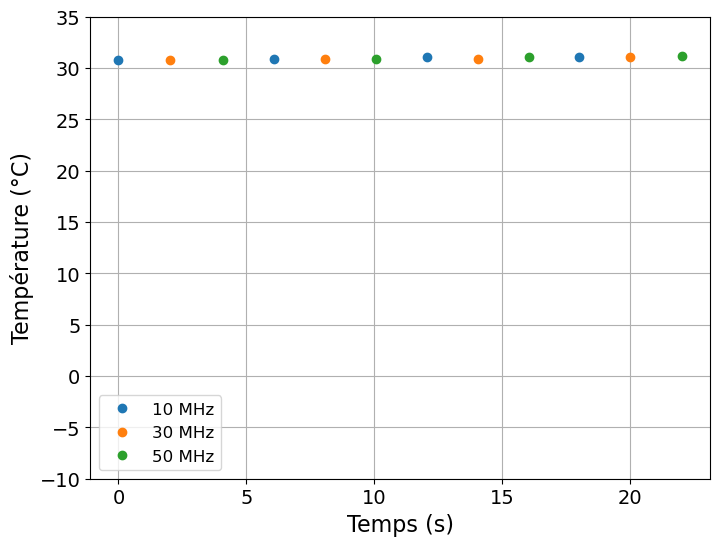
\includegraphics[width=0.8\textwidth]{assets/figures/TempFiltered.png}
    \caption{Fenetre principale du logiciel de mesure}
    \label{fig:TempBruitFiltre}
\end{figure}

Les résultats sont exelenet et la température est stable et ne varie plus de plus de 0.1 degré Celsius, entre les différentes harmoniques.
le filtre passe-bas a donc permis de stabiliser la mesure de température en éliminant les perturbations dues aux fréquences indésirables.

\subsection{Calibration du capteur}
Une calibration est nessecaire pour connaitre la convertion entre la tention en sortie du circuit et la temperature.
Pour ce faire 

\section{Viscosité}
Pour effectuer les mesures de viscosité nous avons d'abord pris des mesures de la réponse fréquentielle du capteur dans plusieurs milieux.
afin de comparer les résultats avec les mesures de viscosité théorique des éléments. Les éléments choisis sont l'air, l'eau distillée, l'éthanol et l'huile moteur.
\begin{table}[H]
    \centering
    \begin{tabular}{|l|c|}
        \hline
        \textbf{Élément}      & \textbf{Viscosité (mPa·s)} \\
        \hline
        Air                  & 0.018 \\
        Eau distillée        & 1.00  \\
        Éthanol              & 1.20  \\
        Huile moteur         & 150   \\
        \hline
    \end{tabular}
    \caption{Viscosité des différents échantillons mesurés à température ambiante}
    \label{tab:viscosite_elements}
\end{table}
Ces échantillons ont été choisis pour leur grande différance de viscosité mais aussi pour leur disponibilité et leur faible dangerosité
Pour ce test le quartz utiliser est un quartz de 5MHz. La cellule Fluidic est utiliser sans pompe et le capteur est rempli de l'echantillon au moyen d'une ceringue. 
Aucun changement de temperature n'est effectuer pendant la mesure, ni aucune mesure de viscosité au moyen du viscomètre au laboratoire.
Ce test a pour vocation de montrer la façon dont la fréquence de résonance change en fonction de la viscosité du milieu dans lequel le quartz est immergé. Et de comparer avec les resultat theorique de viscosité de ces éléments trouvé dans les tables CRM\cite{crm_viscosity_table}.

\section{Gestion de la température}
Avant de pouvoir faire de la gélatine il est essentiel de pouvoir refroidir le liquide à une température en dessous de 20 degrés pour que le processus de gélification commence.
pour cela un bain de glace est utilisé. le liquide est mis dans le récipient en verre du module électrochimique. au moyen d'un tuyau et d'une pompe péristaltique le liquide est circulé autour du récipient. le tuyau est enroulé autour du récipient afin de créer un échangeur de chaleur.
\begin{figure}[H]
    \centering
    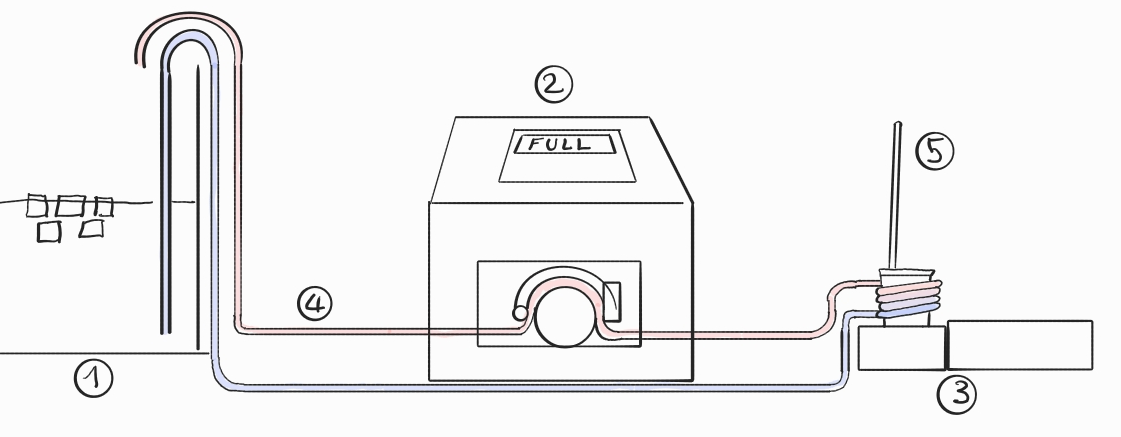
\includegraphics[width=\textwidth]{assets/figures/Pump TB.png}
    \caption{Schéma de refroidissement du module QCM}
    \label{fig:Shema_glacière}
\end{figure}
Afin de chauffer le mélange si une température plus haute que la température ambiante est nécessaire, le bac d'eau glacée est remplacé par un bain chauffant réglable.

Pour tenir le tuyau en place un clip a été designer et imprimer en 3D. le clip est composer de 4 section ce cercle qui permete de glicer le tyeau flexile a l'intreieur mais il ne peut pas sortir facilement.
\begin{figure}[H]
    \centering
    \includegraphics[width=\textwidth]{assets/figures/ATACHE TUBE V2.png}
    \caption{Schéma de refroidissement du module QCM}
    \label{fig:Shema_glacière}
\end{figure}

\section{Gélification}
Les mesures de gélification sont utiles car elles permettent d'observer les transitions de phase d’un état liquide vers un état gélatineux. La gélatine bovine est utilisée car ses changements de phase se produisent à des températures proches de la température ambiante, ce qui correspond bien à la plage de fonctionnement du capteur QCM.

La préparation de la solution consiste à dissoudre la gélatine dans de l’eau chaude. Un rapport de 7,5 g de gélatine pour 100 g d’eau a été utilisé. L’eau est chauffée à 60 °C, puis le mélange est agité pendant 30 minutes afin d’assurer une dissolution complète.

\index{expérience}

Le protocole mis en œuvre pour étudier la gélification est le suivant :
\begin{itemize}
\item Préparer la solution de gélatine comme décrit ci-dessus.
\item Remplir la cellule QCM avec la solution chaude.
\item Démarrer l’acquisition des données à l’aide du capteur QCM.
\item Refroidir progressivement la solution à l’aide du système de refroidissement décrit précédemment.
\item Observer les variations de la fréquence de résonance tout au long du processus de gélification.
\end{itemize}
